\documentclass{article}

% if you need to pass options to natbib, use, e.g.:
%     \PassOptionsToPackage{numbers, compress}{natbib}
% before loading neurips_2019

% ready for submission
% \usepackage{neurips_2019}

% to compile a preprint version, e.g., for submission to arXiv, add add the
% [preprint] option:
%     \usepackage[preprint]{neurips_2019}

% to compile a camera-ready version, add the [final] option, e.g.:
\usepackage[final]{neurips_2019}

% to avoid loading the natbib package, add option nonatbib:
%     \usepackage[nonatbib]{neurips_2019}

\usepackage[utf8]{inputenc} % allow utf-8 input
\usepackage[T1]{fontenc}    % use 8-bit T1 fonts
\usepackage{hyperref}       % hyperlinks
\usepackage{url}            % simple URL typesetting
\usepackage{booktabs}       % professional-quality tables
\usepackage{amsfonts}       % blackboard math symbols
\usepackage{nicefrac}       % compact symbols for 1/2, etc.
\usepackage{microtype}      % microtypography
\usepackage{amsfonts}
\usepackage{amsmath}
\usepackage{graphicx}
\graphicspath{ {./images/} }

\usepackage{amsmath,amssymb,bm}
\usepackage{caption}
\captionsetup[figure]{labelfont=small, justification=centering}
\usepackage{subcaption}
\usepackage{mathtools}
\usepackage{lmodern}
\usepackage{siunitx}
\usepackage{booktabs}
\usepackage{etoolbox}

\DeclarePairedDelimiter\floor{\lfloor}{\rfloor}
\newcommand{\p}{\mathrm{P}}
% Linear Algebra
\newcommand{\vect}[1]{\bm{#1}} % vectors
\newcommand{\matr}[1]{\bm{#1}} % matrices and tensors
\newcommand{\tr}[1]{#1^{\top}} % transpose
\renewcommand{\sp}[2]{#1^{\top}#2}   %scalar product
\renewrobustcmd{\bfseries}{\fontseries{b}\selectfont}
\renewrobustcmd{\boldmath}{}
\newrobustcmd{\B}{\bfseries}

\title{Univariate Time Series Forecasting using ES-RNN and N-BEATS}

% The \author macro works with any number of authors. There are two commands
% used to separate the names and addresses of multiple authors: \And and \AND.
%
% Using \And between authors leaves it to LaTeX to determine where to break the
% lines. Using \AND forces a line break at that point. So, if LaTeX puts 3 of 4
% authors names on the first line, and the last on the second line, try using
% \AND instead of \And before the third author name.
\author{%
  Yves Greatti \\
  New York University\\
  \texttt{yves.greatti@nyu.edu} \\
  % examples of more authors
   \And
    Zian Chen \\
    New York University\\
    \texttt{zian.chen@nyu.edu} \\
    \And 
   Sunjoo Park\\
    New York University\\
    \texttt{sunjoo.park@nyu.edu}
}
\begin{document}

\maketitle

\begin{abstract}
  In this work, we seek to replicate and improve the results reached by two neural networks: \textbf{ES-RNN} and \textbf{N-BEATS} on the M4 dataset competition.
  We also run different experimentations to compare the performances of these two deep learning techniques to a more classical statistical approach like Gaussian Process ($\mathcal{GP}$).
  We demonstrate that although Gaussian processes could be powerful for sampling tasks and simpler to configure, these neural networks outperform it for forecasting. Neural networks could have an overhead in term of the number of hyper-parameters to tune, but when using batching they scale up very easily and generalize well to a large number of time series (100K for M4). We are thus, pretty confident that, the two neural networks could forecast with the appropriate setting of hyper-parameters, other univariate time series beyond the M4 dataset.  
  
 \end{abstract}

\section{Introduction}
\label{Introduction}

The dataset is provided by the M4 competition organized by the International Institute of Forecasters. These competitions also known as the "Makridakis competitions", have been happening since 1982, roughly every 10 years with an increasing number of time series to forecast
starting from 1000 in 1982  to 100,000 in 2018, for the M4 competition. They attract people from academia as well practitioners, the last winner is Slawek Smyl, from Uber Technologies. The model used by Smyl is a hybrid approach combining Holts-Winter smoothing
techniques with a recurrent neural network (RNN). Boris Oreshkin et al. want to challenge the conclusion that, mixed techniques are the future by proposing a pure DL model with interpretable outputs: \textbf{N-Beats}, which they claim outperforms \textbf{ES-RNN}, Smyl's model. N-Beats could be a very deep DL model and it is important for their authors that, in addition to hight accuracy, N-Beats has interpretable outputs which can match established statistical models such as ETS and ARIMA, robust, efficient, and automatic models. 


\section{Problem Description}
\label{problemdescription}
Univariate point forecasting in discrete time consists in predicting future values given a series of observations.
\par\noindent\rule{\textwidth}{0.4pt}
\begin{itemize}
	\item Given an history $[ y_1, \cdots, y_T ]$
	\item TASK: predict $[y_{T+1}, \cdots , y_{T+H} ]$
	\item H: horizon, T: length of observations, m: periodicity of the data
	\item Standard scale-free metrics in the practice of forecasting:
	\begin{itemize}
			\item [--]  sMAPE: symmetric Mean Absolute Percentage Error
			\item [--]  MASE: Mean Absolute Scaled Error
	\end{itemize}
\end{itemize}

For the purpose of this research, we use the predictive accuracy metrics sMAPE and MASE which are the standard metrics used across the forecasting community, 
disregarding $\text{OWA}$ which is a metric defined by Makridakis and requires $\text{MASE}_{\text{Naive2}}$  as part of its computation, which is generated by a random walk model set up by the organizers of the competition.

\[
	\text{sMAPE} = \frac{2}{H}  \sum_{i=1}^{H} \frac{ | y_{T+i}  - \hat{y}_{T+i} | } { | y_{T+i} | + | \hat{y}_{T+i} | } \text{ ,     } 
	\text{MASE} = \frac{1}{H}  \sum_{i=1}^{H} \frac{ | y_{T+i}  - \hat{y}_{T+i} | } { \frac{1} {T + H - m} \sum_{j=m+1}^{T+H}  | y_j  - y_{j-m} | }
\]



\subsection{Data Description}
\label{datadescription}

M4 dataset extends the previous three competitions by increasing significantly the number of series. The time series are grouped into six categories and can be split into two groups: 
high-frequency data (weekly, daily, hourly) along with low-frequency data (yearly, quarterly and monthly).  They were built from real, multiple, and diverse sources and are divided into six data types:
demographic, finance, industry, macro, micro and other. The minimum of observations for the training set are 79 for hourly, 652 for daily, 67 for weekly, 24 for monthly, 8 for quarterly and 7 for yearly series.
They have different length raging from 7 to about 1000 observations.

\begin{table}[!ht]
	\centering
  	\begin{tabular}{cccccccc} \toprule
		\textbf{Frequency} & \textbf{Demographic} & \textbf{Finance} & \textbf{Industry} & \textbf{Macro} & \textbf{Micro} & \textbf{Other} & \textbf{Total}  \\ \midrule
		Yearly & 1,088 & 6,519 & 3,716 & 3,903 & 6,538 & 1,236 & 23,000 \\
		\midrule
		Quarterly & 1,858 & 5,305 & 4,637 & 5,315 & 6,020 & 865 & 24,000 \\
		\midrule
		Monthly & 5,728 & 10,987 & 10,017 & 10,016 & 10,975 & 277 & 48,000 \\
		\midrule		
		Weekly & 24 & 164 & 6 & 41 & 112 & 12 & 359 \\
		\midrule		
		Daily & 10 & 1,559 & 422 & 127 & 1,476 & 633 & 4,227 \\
		\midrule		
		Hourly & 0 & 0 & 0 & 0 & 0 & 414 & 414 \\
		\midrule		
		Total & 8,708 & 24,534 & 18,798 & 19,402 & 25,1212 & 3,437 & 100,000 \\
		 \bottomrule
	\end{tabular}
	\caption{M4 data by type and series frequency}
	\label{tab:dsstats}
\end{table}

\begin{table}[!ht]
	\centering
  	\begin{tabular}{cccccccc} 
		\toprule
			& \textbf{Mean} & \textbf{Std-Dev} & \textbf{Min} & \textbf{25\%} & \textbf{50\%} & \textbf{75\%} & \textbf{Max}  \\ 
		\midrule
		Yearly & 25 & 24 & 7 & 14 & 23 & 34 & 829 \\
		\midrule
		Quarterly & 84 & 51 & 8 & 54 & 80 & 107 & 858 \\
		\midrule
		Monthly & 198 & 137 & 24 & 64 & 184 & 288 & 2776 \\
		\midrule		
		Weekly & 1009 & 707 & 67 & 366 & 921 & 1590 & 2584 \\
		\midrule		
		Daily & 2343 & 1756 & 79 & 309 & 2926 & 4183 & 9905 \\
		\midrule		
		Hourly & 805 & 127 & 652 & 652 & 912 & 912 & 912 \\
    	       \bottomrule
	\end{tabular}
	\caption{M4 series length statistics}
	\label{tab:dslengthstats}
\end{table}


\section{ES-RNN}
\label{ESRNN}

\subsection{Model Description}

ES-RNN algorithm consists in two major layers: a preprocessing layer which uses Holt-Winter smoothing technic to extract trend and seasonality parameters and a dilated RNN network.
The Holt-Winter parameters are part of the back-propagation and are tuned as the network learns the characteristics of the time series. The ES-RNN model uses a modified version of the Holt-Winters formula,
in which there is no local linear level coefficient, and level and seasonality terms are scaled instead of subtracted. 
The linear forecast is replaced by an RNN, which has for input the normalized and de-seasonalized prior observations. 


\begin{align*}
	l_t 	&= \alpha \frac{y_t} {s_{t-m}} + (1-\alpha) l_{t-1} \\
	s_t 	&= \beta \frac{y_t}{l_{t-1}} + (1-\beta) s_{t-m} \\
	\hat{y}_{\textbf{win}}		&= \textbf{ES-RNN}(\frac{y_{ti}}{s_{ti} l_{ti}}) \\
	y_{\textbf{truth}}		&= (\frac{y_{to}}{s_{to} l_{to}}) 
\end{align*}
where $l$ is a state variable, $s$ is a seasonality coefficient, $\alpha$ and $\beta$ are network parameters, $m$ is the periodicity of the data.

To model long-term dependencies in time series, ES-RNN uses dilated RNNs which allow to stack RNN cells by having skip connections between RNN cells . 
The dilation parameters  are given in table \autoref{tab:dilations}.  DRNN cells can be vanilla RNN, LSTM, GRU,  GRU cells provides the higher accuracy.

\begin{table}[!ht]
	\centering
	\begin{tabular}{clclc} \toprule
		\textbf{Time Series} & \textbf{Dilations} \\ 
		\midrule
		Quarterly  & (1, 2), (4, 8)	\\
		\midrule
		Monthly 	& (1, 3), (6, 12)	\\
		\midrule
		Daily 	& (1, 7), (14, 28)	\\
		\midrule		
		Yearly 	& (1, 2), (2, 6) 	\\
		\midrule		
		Weekly 	& (1, 14), (14, 28)	\\
		\midrule		
		Hourly 	& (1, 24), (24, 48)	\\
	\end{tabular}
	\caption{ES-RNN dilation parameters}
	\label{tab:dilations}
\end{table}


 \subsection{Data Preparation}
 The M4 time series have different length, to allow vectorization and to take advantage of the GPUs, they are chopped using a predetermined cut off value.
 To the exception of the daily time series, for which the cut-off value is 200, 72 is used as the default value (\autoref{tab:cutoff}).
 
 \begin{table}[!ht]
	\centering
	\begin{tabular}{llllllll} 
	\toprule
		& \multicolumn{6}{c} {\textbf{Filtering rates (in \%)}} \\
			& \textbf{Hourly} & \textbf{Daily} & \textbf{Weekly} & \textbf{Monthly} & \textbf{Quarterly}   & \textbf{Yearly} \\
		\midrule
		 	& 6.93 	& 6.93  & 18.11 & 26.83 &  45.42 & 60.61 \\
		\bottomrule
	\end{tabular}
	\caption{Percentage of time series eliminated by the cut-off value}
	\label{tab:cutoff}
\end{table}


 The batch size is by default 1024, we observe that, it has no effects on the overall performance of the network.
 
 For an hourly frequency, the effect of the batch size is given in table  \autoref{tab:batchsize} .
 \begin{table}[!ht]
	\centering
	\begin{tabular}{llllllll} \toprule
			& \multicolumn{6}{c} {\textbf{sMAPE per category}} \\
		\textbf{Batch size} & \textbf{Demographic} & \textbf{Finance} & \textbf{Industry} & \textbf{Macro} & \textbf{Micro} & \textbf{Other} & \textbf{Total}  \\ \midrule
		512 & 6.32 & 3.34 & 3.95 & 2.52 & 2.43 & 3.08 & 3.02 \\
		\midrule
		1024 & 6.20 & 3.27 & 3.9 & 2.52 & 2.37 & 3.07 & 2.97 \\
		\midrule
		2048 & 6.26 & 3.32 & 3.92 & 2.49 & 2.42 & 3.1 & 3.01 \\
		 \bottomrule
	\end{tabular}
	\caption{ES-RNN batch size statistics}
	\label{tab:batchsize}
\end{table}
 
 Each time series is split into two windows: a backcast and forecast window.  Observations in each window are normalized and de-seasonalized using the coefficients of the exponential smoothing.
 In addition, a one-hot representation of the time series category is added to the input window.
 
 \begin{figure}[ht]
\centering
	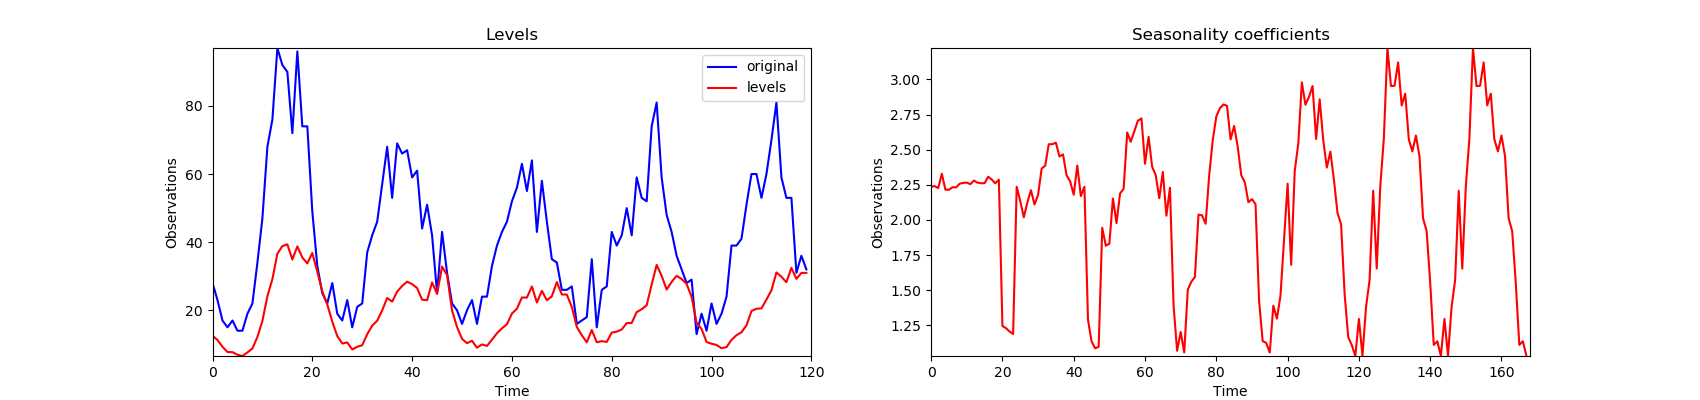
\includegraphics[width=0.9\columnwidth]{H344_levels_seasonalities.png} 
\caption{Levels are a smoothing version of the original time series and \\ seasonality coefficients are between 0 and 1.}
\label{fig:levelsseasonality}
\end{figure}

\begin{figure}[ht]
\centering
	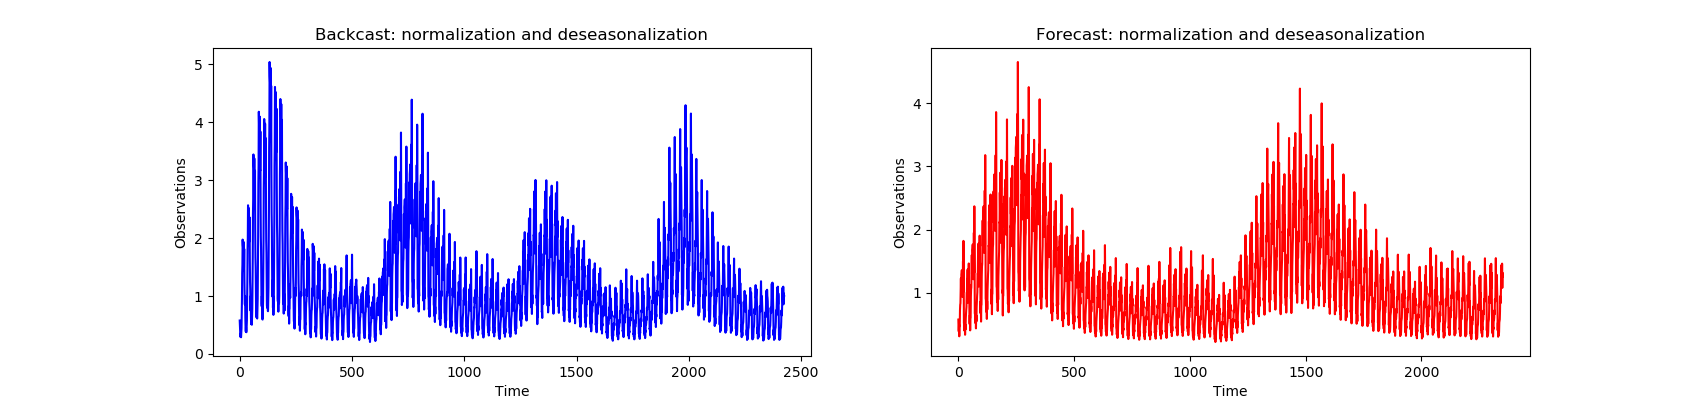
\includegraphics[width=0.9\columnwidth]{H344_windows.png} 
\caption{The input and ouput of the RNN are normalized and de-seasonalized, compared to N-BEATS which are not scaled.}
\label{fig:normalizeddeseasonalized}
\end{figure}

\subsection{Deep learning architecture}

ES-RNN layers from top to bottom consist in a stack of dilated RNNs followed by a fully connected layer, an activation function and a dense layer.

 \begin{table}[!ht]
	\centering
	\begin{tabular}{llllllll} 
		\midrule
			\multicolumn{7}{c} {\textbf{ES-RNN}} \\
		\midrule
			\multicolumn{7}{c} {time series $\in \mathbb{R}^{b \times l}$} \\
		\midrule
			\multicolumn{7}{c} {RNN  $\in \mathbb{R}^{l \times s}$} \\		
		\midrule
			\multicolumn{7}{c} {RNN  $\in \mathbb{R}^{s \times s}$} \\		
		\midrule
			\multicolumn{7}{c} {$\cdots$} \\		
		\midrule
			\multicolumn{7}{c} {RNN  $\in \mathbb{R}^{s \times s}$} \\		
		\midrule
			\multicolumn{7}{c} {dense  $\in \mathbb{R}^{s \times s}$} \\		
		\midrule
			\multicolumn{7}{c} {Tanh} \\		
		\midrule
			\multicolumn{7}{c} {dense  $\in \mathbb{R}^{s \times h}$} \\		
		\midrule
	\end{tabular}
	\caption{ES-RNN architecture. Let $b$ the batch size, l the length of the time series, s the embedding dimensional state size and h the length of the prediction.}
	\label{tab:esrnnarchitecture}
\end{table}


Dropout or batch normalization did not provide any significant improvement, the smoothing and normalization of the data seemed enough for a convergence to a local minimum.
In both networks, using the pinball loss function brought definitely a boost in performance compared to L2 or L1 losses. The pinball loss function is popular in forecasting. 
Two different slopes are used depending whether the forecast $\hat{y}_t$ value is greater
or smaller than the truth value $y_t$. Two models are then trained, corresponding to the lower and upper bounds of the desired level of prediction interval:
\[
	L_\alpha = 
	\begin{cases}
		\alpha (\hat{y}_t  - y_t) & \text{ if } \hat{y}_t \geq y_t \\
		(1-\alpha) (y_t - \hat{y}_t) & \text{ if }  y_t > \hat{y}_t
	\end{cases}
\]
Then $\p(\hat{y}_{t, lower} \le y_t < \hat{y}_{t, upper}) = 1 - 2 \alpha$.
\begin{figure}[ht]
\centering
	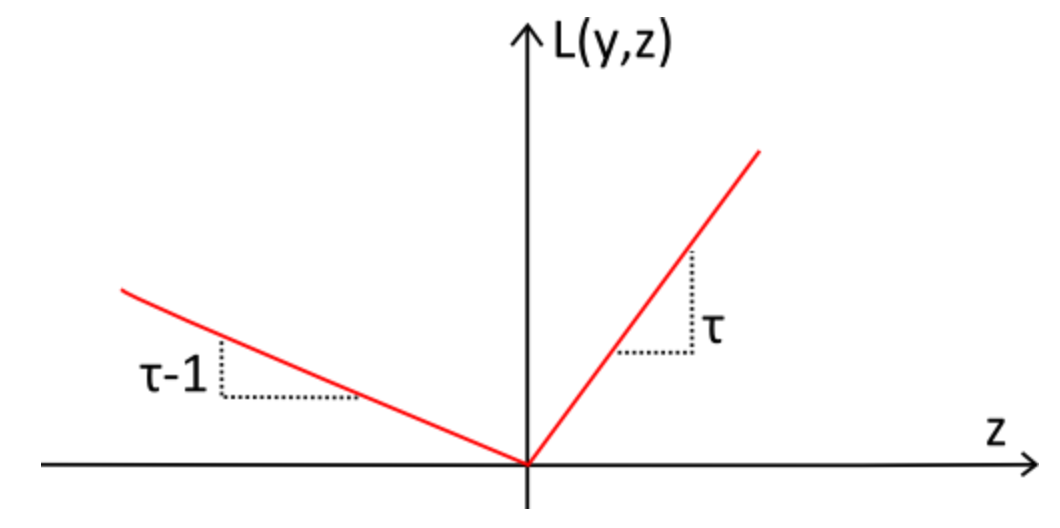
\includegraphics[width=0.4\columnwidth]{pinballloss.png} 
\caption{$\tau$ controls the desired imbalance in the quantile forecast.}
\label{fig:pinballloss}
\end{figure}

\subsection{Training of the network}

Most of the parameters set by Smyl in his initial model are preserved and result in good performances. 
The only changes we made was regarding the learning rate value and that we used a learning rate scheduler.  All experiments for ES-RNN were made 
using Adam. We trained for 100 epochs starting with a learning rate of 0.01 which was progressively reduced to $1 \times 10^{-5}$.
We also changed the batch size as detailed in the previous section and replaced the Tanh activation function with ReLu and LeakyReLu without noticeable improvements.


\section{N-BEATS}
\label{NBEATS}

\subsection{Model Description}
N-Beats architecture by design is simple and generic, yet expressive (deep). It does not rely on any time-series specific feature engineering or input scaling.
It is also extendable and the basic components are:
\begin{itemize}
 	\item[-]  \textbf{Block}
 	\paragraph{} A block accepts an input $\vect{x}$ which is a history lookback window, also known as "backcast". And the block outputs two vectors $\hat{\vect{x}}$ and $\hat{\vect{y}}$,  $\hat{\vect{x}}$ is the block's best estimate
	of $\vect{x}$, $\hat{\vect{y}}$ is the block's forward forecast of length $H$. The length of the input window is a multiple of the forecast horizon $H$, and $\vect{x}$ value range is 2$H$ to 7$H$. Each block removes the portion of the signal
	it can explain well, making the forecast job of the downstream blocks easier.  This also facilitates more fluid gradient backpropagation.
	\item[-]  \textbf{Stack}
	\paragraph{} A stack is a collection of blocks and stacks can be hierarchically organized to make a very deep architecture. Each block provides a partial forecast that is first aggregated at the stack level and then at the overall network level.
 \end{itemize}

\begin{figure}[!ht]
\centering
	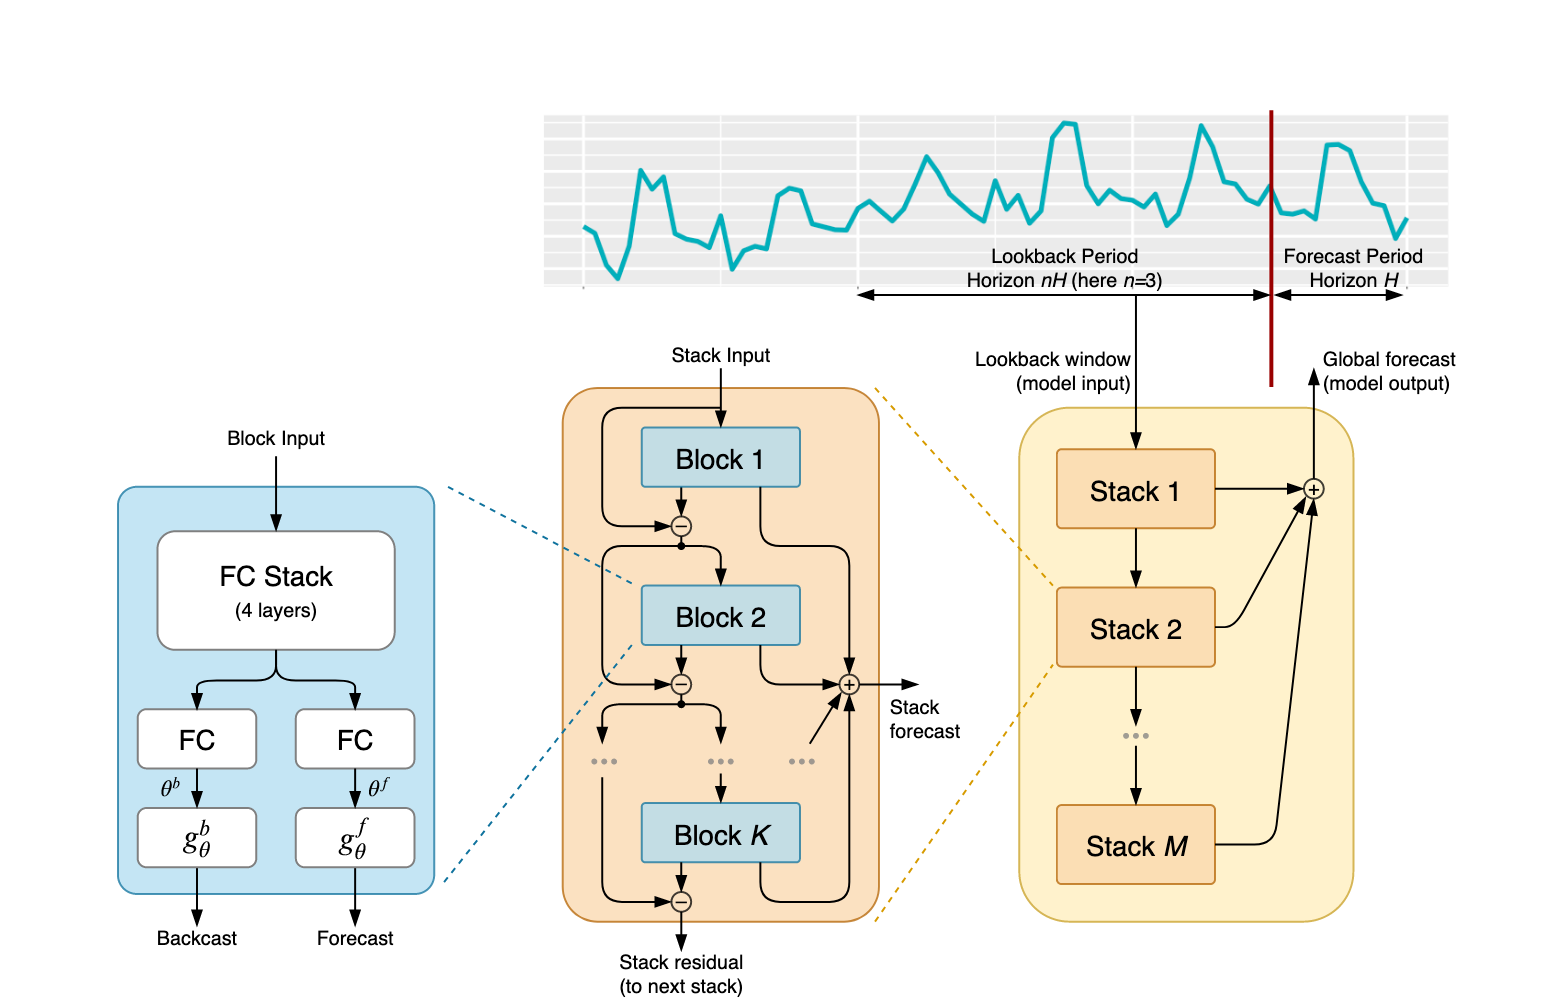
\includegraphics[width=0.6\columnwidth]{n-beats_stack.png} 
\caption{N-BEATS overall architecture.}
\label{fig:nbeatsstack}
\end{figure}

\subsection{Additional model details}
The input $\vect{x}$ goes first through four linear layers followed by two interpolation functions, one for backcast: $g_\theta^b$ and the other for forecast: $g_\theta^f$.
There are three types of blocks:
\paragraph{generic}: $\hat{\vect{y}}_{i,j} = \matr{W}_{i,j} \theta_{i,j} + \vect{b}_{i,j}$. This block outputs are not interpretable.
\paragraph{trend model}: the interpolation is a monotonic function, a polynomial of small degree $p$: \\
$g_\theta = \sum_{i=0}^p \theta_i t^i$ where $\vect{t} = [0,1,2,\cdots,H-2, H-1]^T/H \text{ and p} \le 4$. \\
The trend forecast has the form: 
\[
	\hat{\vect{y}}_{i,j}^{tr} = \matr{T} \theta_{i,j}
\]
The number of  $\theta$ parameters is less or equal to 10.
\paragraph{seasonality model}: to capture cyclical, recurring patterns, this block performs a Fourier transform of the series: 
\begin{align*}
		g_\theta (t)		&= \sum_{i=0}^{\floor*{H/2-1}} \theta_i \cos{(2 \pi it)} + \theta_{i + \floor*{H/2}}  \sin{(2 \pi it)} \\
						&	\text{ where } \theta_{i,j} \text{ are Fourier coefficients predicted by a FC network of layer} j \text{ of stack } i \\
		\hat{\vect{y}}_{i,j}^{s} &= \matr{S} \theta_{i,j}		
\end{align*}
The weight could be shared among the blocks within the same stack and resulted in better performance of the validation set.

\begin{table}[!ht]
	\centering
	\begin{tabular}{llllllll} 
		\midrule
			\multicolumn{7}{c} {\textbf{N-BEATS}} \\
		\midrule
			\multicolumn{7}{c} {time series $\in \mathbb{R}^{b \times W \times bc}$} \\
		\midrule
			\multicolumn{7}{c} {FC  $\in \mathbb{R}^{bc \times s}$} \\		
		\midrule
			\multicolumn{7}{c} {ReLU} \\		
		\midrule
			\multicolumn{7}{c} {FC  $\in \mathbb{R}^{s \times s}$} \\		
		\midrule
			\multicolumn{7}{c} {ReLU} \\		
		\midrule
			\multicolumn{7}{c} {FC  $\in \mathbb{R}^{s \times s}$} \\		
		\midrule
			\multicolumn{7}{c} {ReLU} \\		
		\midrule
			\multicolumn{7}{c} {backcast = $g_\theta^b(x)$} \\		
			\multicolumn{7}{c} {forecast = $g_\theta^f(x)$} \\		
		\midrule
	\end{tabular}
	\caption{N-BEATS architecture. Let $b$ the batch size, W is the number of input windows, bc backcast length, s is the size of the hidden layer.}
	\label{tab:nbeatsstack}
\end{table}

\subsection{Training of the network}
We split data into training and validation and test datasets, similarly to what we did for ES-RNN model, the only difference is that we dynamically determined the cut-off value by selecting the minimal size of the time series which
are larger than the minimum length: backcast + forecast. We run various experiments with different configuration of the stacks, number of blocks per stack, 
size of the hidden layer, the batch size and values  for the $\theta$ parameters.  We also trained the network for 100 epochs with an initial learning rate of 0.01,
 which was progressively reduced by the scheduler to $1 \times 10^{-7}$.

 The batch size is by default 1024, we observe that, it affects the overall performance of the network, depending the time series frequency,
 too small the validation loss jumped up and down, and with larger batch size, the performance was better.
 In addition, using dropout with a value of 0.,2 helps to have a good accuracy.

Oreshkin et al. claimed that their model is interpretable when looking at the outputs of the trend or seasonality blocks. We did not obtain exactly the same results, and this is maybe due to the fact we did not
do ensembling neither that we have a very deep architecture. They had 6 models for each time series category,  a very deep network of total depth 150 layers, trained each model on input windows of
different length: $2H,3H, \cdots, 7H$ and followed a bagging procedure four 180 models.

\begin{figure}[ht]
\centering
	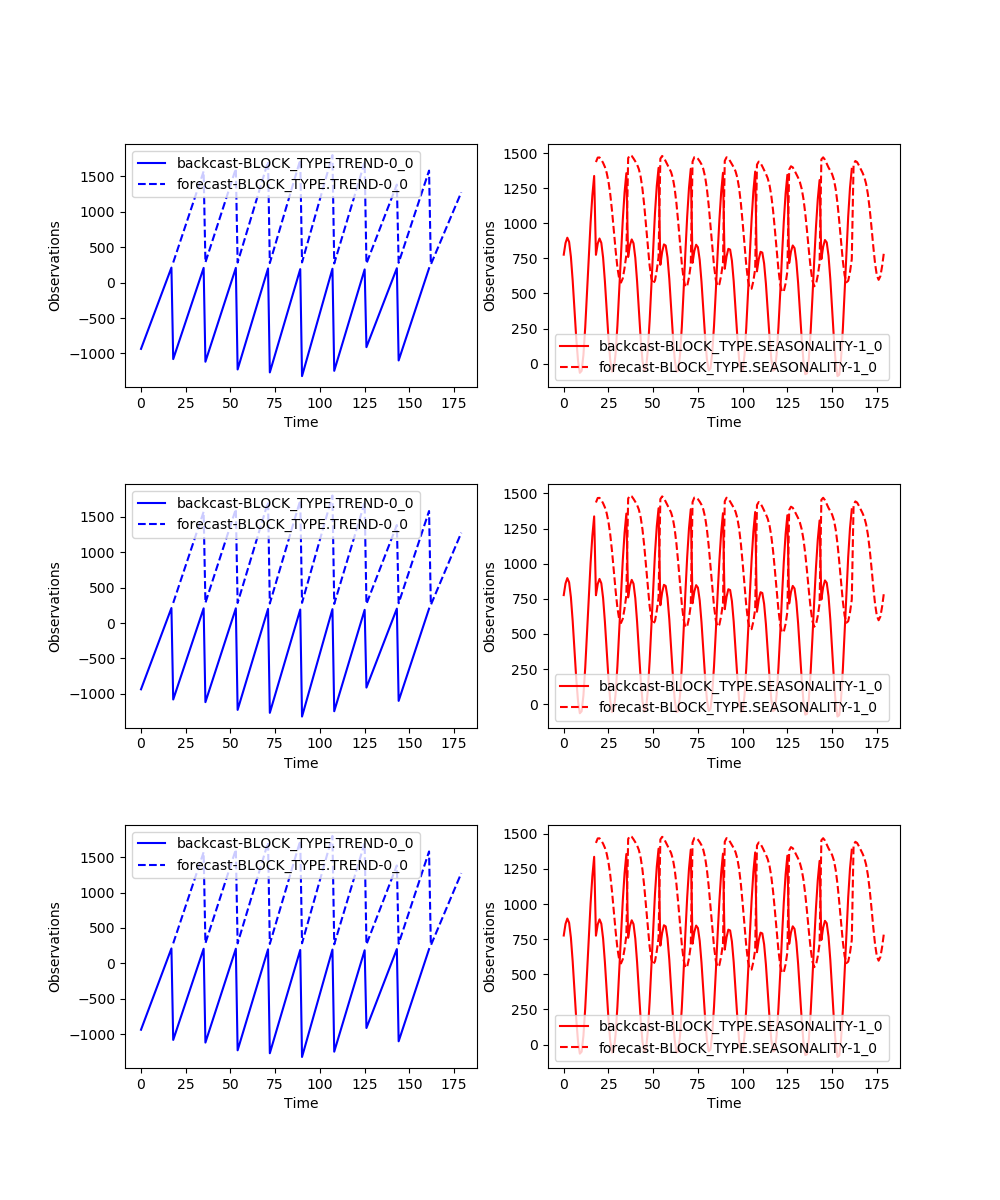
\includegraphics[width=0.8\columnwidth]{M1_stack_reload_100.png} 
\caption{Trend and seasonal coefficients for the backcast and forecast outputs of the M1 time series.}
\label{fig:m1trendseasonality}
\end{figure}


\section{Model comparison}
\label{modelcomparison}

We used ARIMA and Gaussian Process to generate our baselines. ARIMA was one of the method used by the M4 competition organizers to generate the benchmarks.
We also decided to use $\mathcal{GP}$ for their simplicity, the possibility to select different kernels and the possibility to have confidence intervals related to theirs forecasting.
On a single time series traditional statistical models like ARIMA are difficult to outperform, the downside is that they do not scale up with the number of time series, since each time series require to carefully
tune the (p,q,d) parameters. ES-RNN seemed to perform better than N-BEATS but requires more tuning and go deeper in the number of layers.

\begin{table}[!ht]
	\centering
	\begin{tabular}{lllllll} 
		\toprule
		& \multicolumn{6}{c} {\textbf{sMAPE by Frequency}} \\
		\textbf{Model} & \textbf{H344} & \textbf{D1} & \textbf{W246} & \textbf{M1} & \textbf{Q66} & \textbf{Y1}  \\
		\midrule
		ARIMA & \B 23.24 & \B 0.28 & \B 5.51 & 30.40 & 5.96 & 11.20 \\
		\midrule
		GP  & 94.93	&  22.37 & 32.7	 & 19.04 & 35.02 & 20 \\
		\midrule
		ES-RNN 	& 36.68 	& 6.48  & 23.44 & \B 10.19 & 10.2 & \B 1.99 \\
		\midrule
		N-BEATS 	& 43.98 	& 6.54 & 30.83 & 24.68	&  \B 1.47 & 9.53 \\
		 \bottomrule
	\end{tabular}
	\caption{Comparison of results on specific time series, in bold the best score, the lower the better.}
	\label{fig:modelcomparision}
\end{table}

\begin{table}[!ht]
	\centering
	\begin{tabular}{llllllll} 
	\toprule
		& \multicolumn{6}{c} {\textbf{sMAPE by Frequency}} \\
		\textbf{Model} & \textbf{Hourly} & \textbf{Daily} & \textbf{Weekly} & \textbf{Monthly} & \textbf{Quarterly}   & \textbf{Yearly} \\
		\midrule
		ES-RNN 	& 30.26 	& \B 2.97  & 14.84 & \B 9.78 &  10.51 & 14.58 \\
		\midrule
		N-BEATS 	&  20.1 & 4.08 & 16.05 & 22.22	& 11.94 & 13.12 \\
		\bottomrule
	\end{tabular}
	\caption{Performance on the M4 test set, in bold when the models performed better than in the original papers.}
		\label{fig:esrnnnbeatsdiff1}
\end{table}

\begin{table}[!ht]
	\centering
	\begin{tabular}{cccc}
	 \toprule
		\textbf{Data Category} & \textbf{Yearly} & \textbf{Quarterly} & \textbf{Monthly} \\
		Demographic &  \B 11.45 & 11.67 & \B 5.76 \\
		\midrule
		Finance & \B 16.31 & \B 10.41 & \B 10.8 \\
		\midrule
		Industry & 21.98 & 8.74 & \B 11.3 \\
		\midrule
		Macro & \B 14.21 & 10.13& \B 11.7 \\
		\midrule
		Micro & \B 10.93 & 11.96 & \B 8.02 \\
		\midrule
		Other & 16.27 & 7.87 & \B 7.76 \\
		\midrule
		Overall & 14.58 & 10.51 & \B 9.78 \\		
		\bottomrule
	\end{tabular}
	\caption{ES-RNN: breakdown of sMAPE by time period and category}
\end{table}

\begin{table}[!ht]
	\centering
	\begin{tabular}{cccc}
	 \toprule
		\textbf{Data Category} & \textbf{Yearly} & \textbf{Quarterly} & \textbf{Monthly} \\
		Demographic &  10.34 & 11.74 & 5.57 \\
		\midrule
		Finance & 14.11 & 13.90 & 15.36 \\
		\midrule
		Industry & 17.16 & 10.85 & 14.76 \\
		\midrule
		Macro & 13.39 & 11.35 & 14.6 \\
		\midrule
		Micro & 10.92 & 12.22 & 15.2 \\
		\midrule
		Other & 13.62 & 7.90 & 13.89 \\
		\midrule
		Overall & 13.29 & 11.94 & 13.88 \\		
		\bottomrule
	\end{tabular}
	\caption{N-BEATS: breakdown of sMAPE by time period and category}
\end{table}

\newpage

\begin{figure}[!h]
  \centering
  \begin{tabular}[c]{cc}
    \begin{subfigure}[c]{0.6\textwidth}
      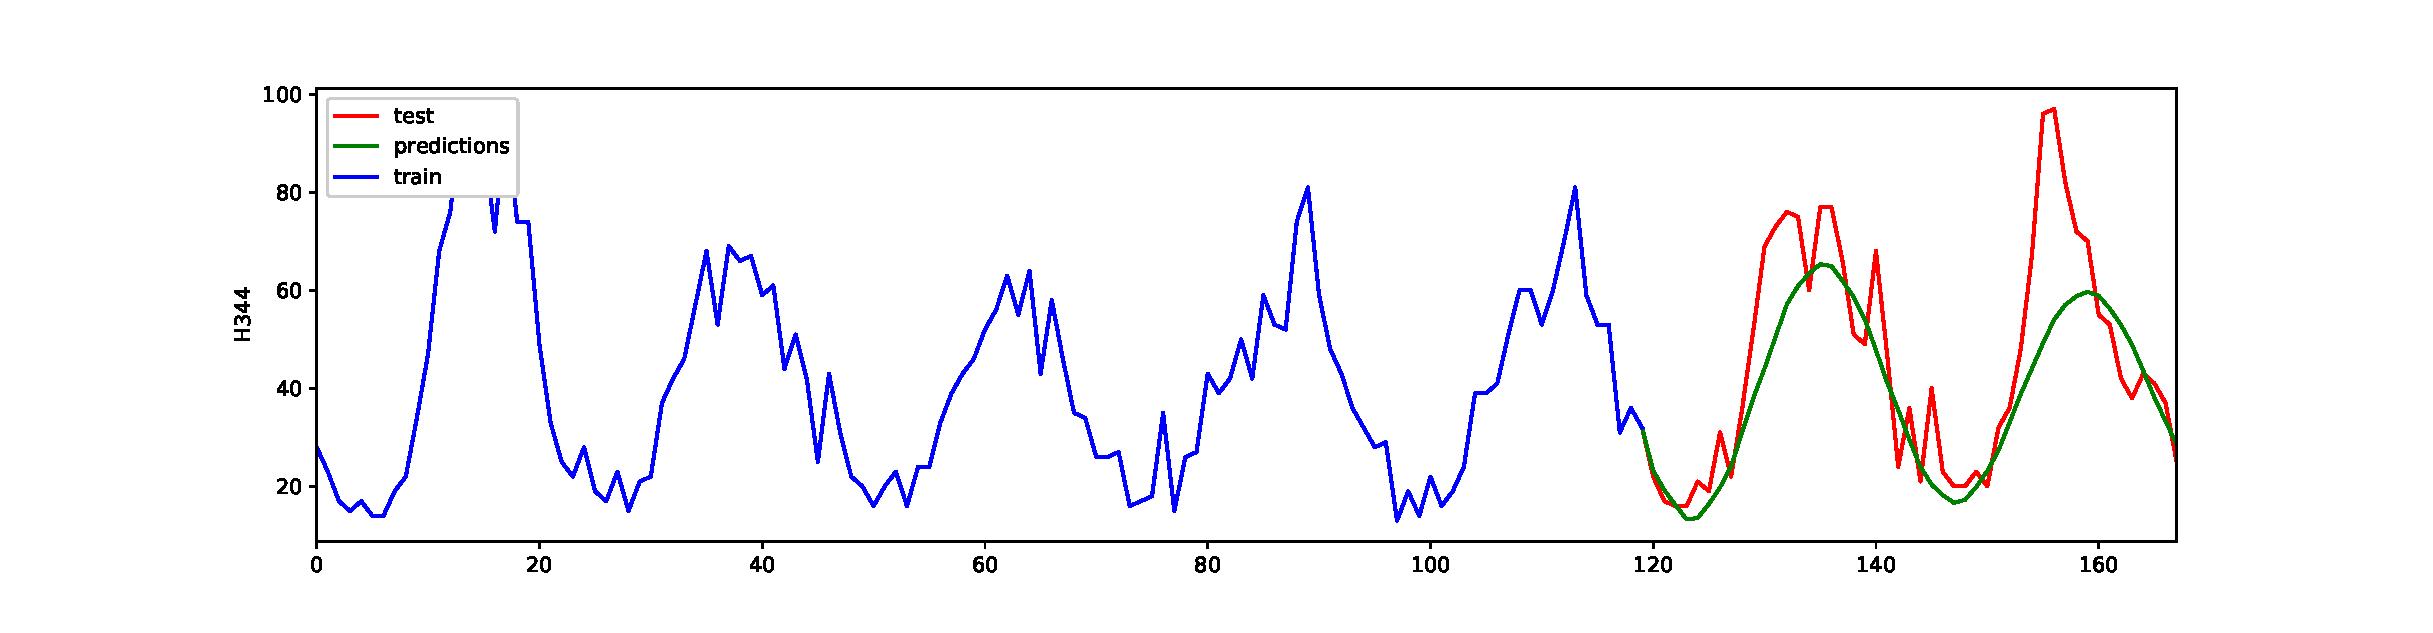
\includegraphics[width=\textwidth]{H344_ARIMA.eps}
      \caption{ARIMA predictions for H344}
      \label{fig:stackpred1}
    \end{subfigure}&
    \begin{subfigure}[c]{0.6\textwidth}
      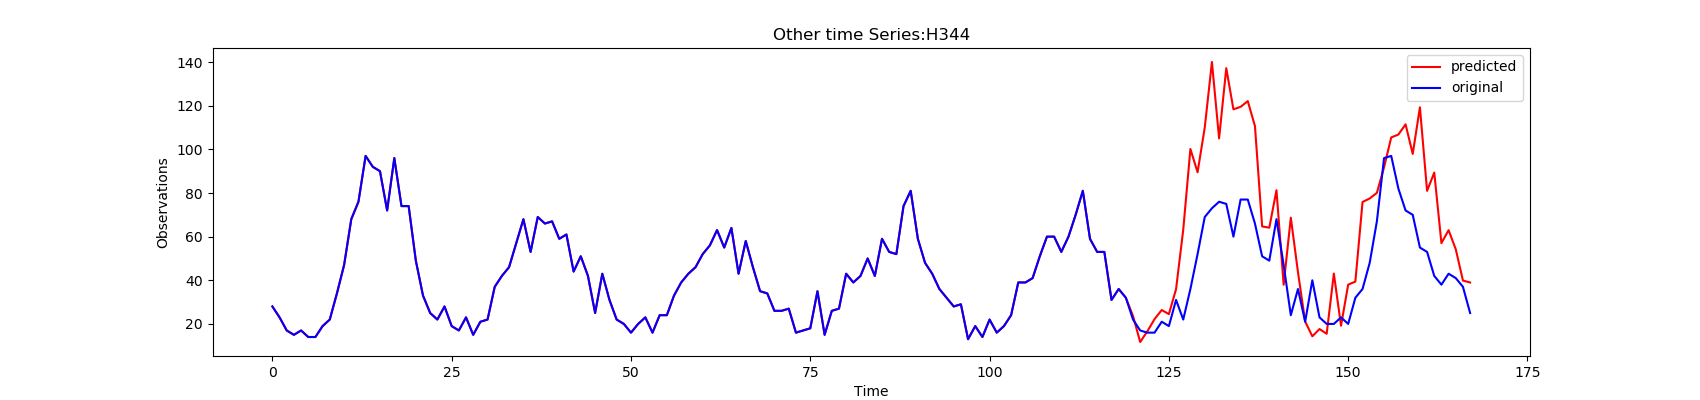
\includegraphics[width=\textwidth]{H344_esrnn_time_series.png}
      \caption{ES-RNN predictions for H344}
      \label{fig:stackpred2}
    \end{subfigure}\\
    \begin{subfigure}[c]{0.5\textwidth}
      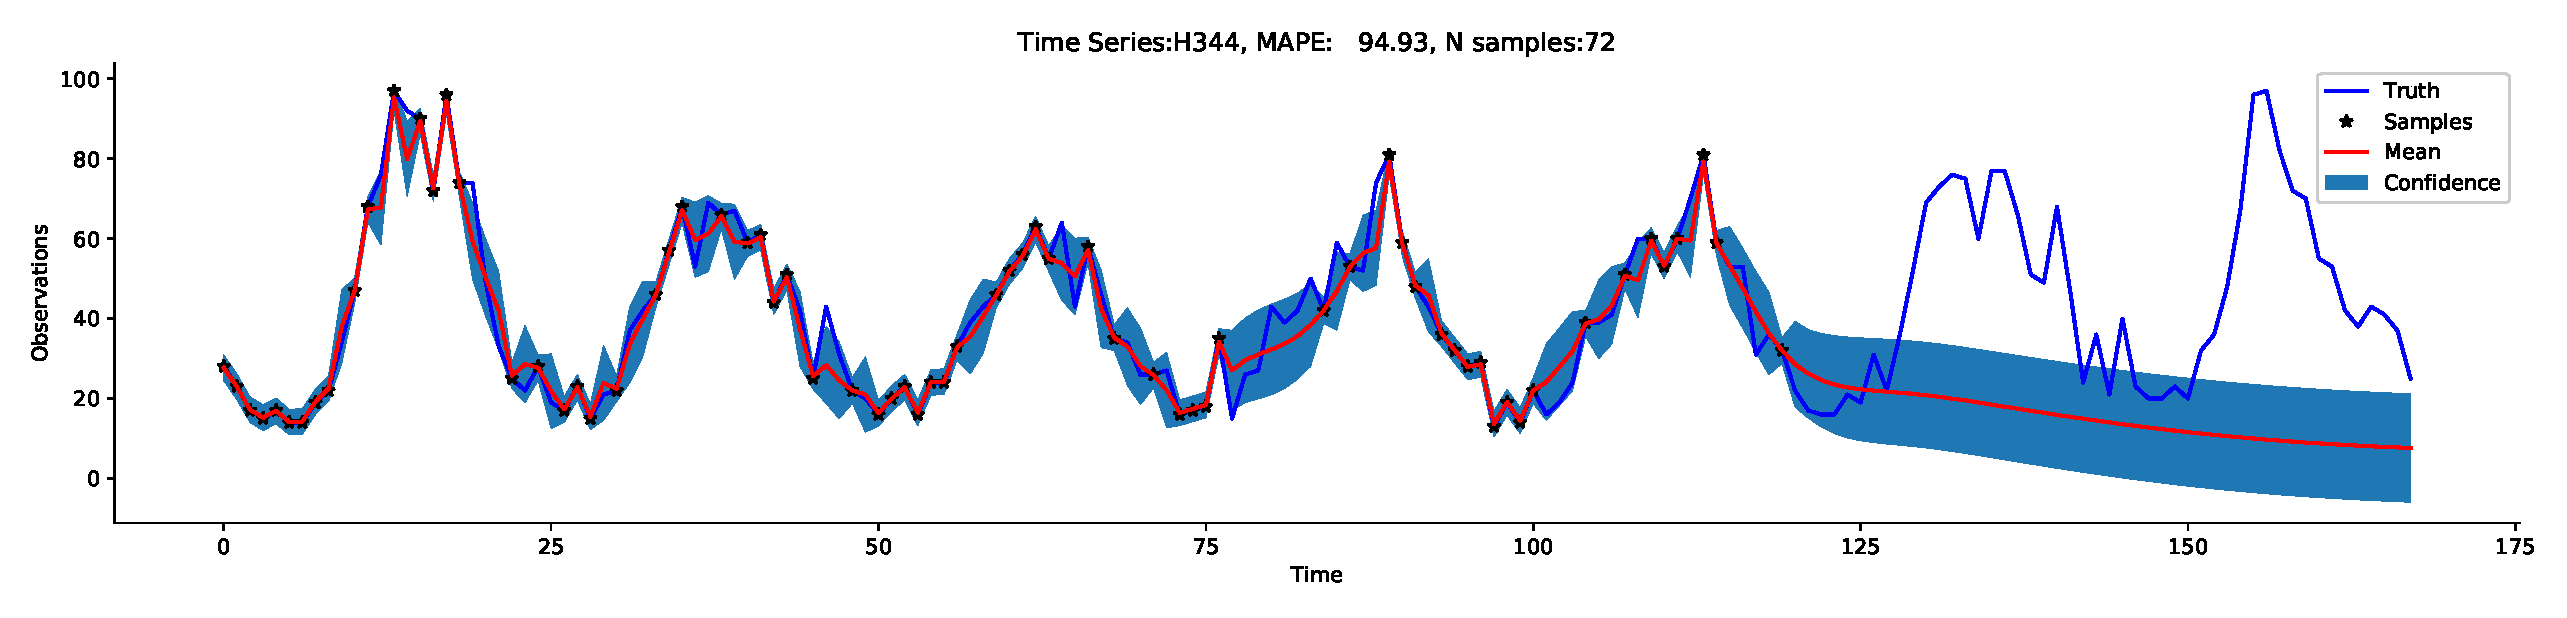
\includegraphics[width=\textwidth]{H344_GP_time_series.eps}
      \caption{GP predictions for H344}
      \label{fig:stackpred3}
    \end{subfigure}&
    \begin{subfigure}[c]{0.6\textwidth}
      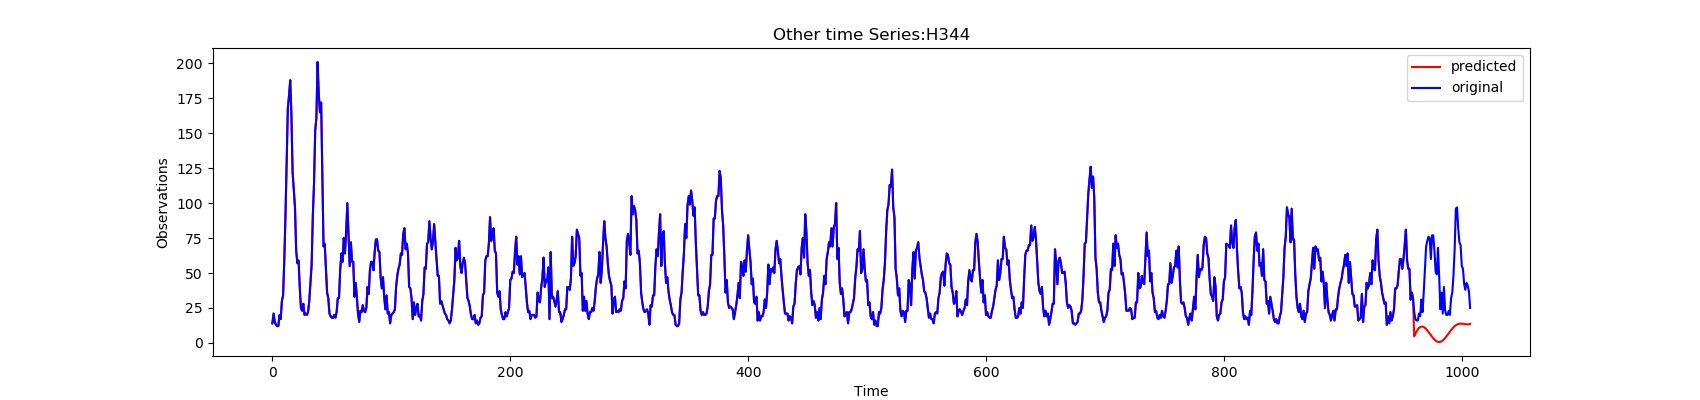
\includegraphics[width=\textwidth]{H344_nbeats_time_series.png}
      \caption{N-BEATS predictions for H344}
      \label{fig:stackpred4}
    \end{subfigure}\\
  \end{tabular}    
  \caption{Predictions for H344 time series: ARIMA (top-left), ES-RNN (top-right), \\ GP (bottom-left), , N-BEATS (bottom-right)}
  \label{fig:stackpred}
\end{figure}


\section*{References}

References follow the acknowledgments. Use unnumbered first-level heading for
the references. Any choice of citation style is acceptable as long as you are
consistent. It is permissible to reduce the font size to \verb+small+ (9 point)
when listing the references. {\bf Remember that you can use more than eight
  pages as long as the additional pages contain \emph{only} cited references.}
\medskip

\small

[1] Alexander, J.A.\ \& Mozer, M.C.\ (1995) Template-based algorithms for
connectionist rule extraction. In G.\ Tesauro, D.S.\ Touretzky and T.K.\ Leen
(eds.), {\it Advances in Neural Information Processing Systems 7},
pp.\ 609--616. Cambridge, MA: MIT Press.

[2] Bower, J.M.\ \& Beeman, D.\ (1995) {\it The Book of GENESIS: Exploring
  Realistic Neural Models with the GEneral NEural SImulation System.}  New York:
TELOS/Springer--Verlag.

[3] Hasselmo, M.E., Schnell, E.\ \& Barkai, E.\ (1995) Dynamics of learning and
recall at excitatory recurrent synapses and cholinergic modulation in rat
hippocampal region CA3. {\it Journal of Neuroscience} {\bf 15}(7):5249-5262.

\end{document}
